\documentclass[14pt]{beamer}
\usepackage[T2A]{fontenc}
\usepackage[utf8]{inputenc}
\usepackage[english,russian]{babel}
\usepackage{amssymb,amsfonts,amsmath,mathtext}
\usepackage{cite,enumerate,float,indentfirst}
\usepackage{booktabs}

\graphicspath{{images/}}

\usetheme{Pittsburgh}
\usecolortheme{whale}

\setbeamercolor{footline}{fg=gray}
\setbeamertemplate{footline}{
  \leavevmode%
  \hbox{%
  \begin{beamercolorbox}[wd=.333333\paperwidth,ht=2.25ex,dp=1ex,center]{}%
    Куликов А.В., ABBYY-MIPT
  \end{beamercolorbox}%
  \begin{beamercolorbox}[wd=.333333\paperwidth,ht=2.25ex,dp=1ex,center]{}%
    Москва, 2017
  \end{beamercolorbox}%
  \begin{beamercolorbox}[wd=.333333\paperwidth,ht=2.25ex,dp=1ex,right]{}%
  Стр. \insertframenumber{} из \inserttotalframenumber \hspace*{2ex}
  \end{beamercolorbox}}%
  \vskip0pt%
}

\newcommand{\itemi}{\item[\checkmark]}

\title{\small{Японский: буквенные n-граммы для распознавания}}
\subtitle{\footnotesize{Контроль НИР}}
\author{\small{%
~Куликов А.В., гр. 397\\%
\emph{Руководитель:}~Андрианов А.И.}\\%
\vspace{30pt}%
ABBYY-MIPT%
\vspace{20pt}%
}
\date{\small{Москва, 2017}}

\begin{document}

\maketitle

\begin{frame}

\frametitle{Задача}
\begin{itemize}
    \item Japanese kanji/kana OCR.
    \item Существуют путающиеся символы, например:
    \begin{figure}[h]
        \center{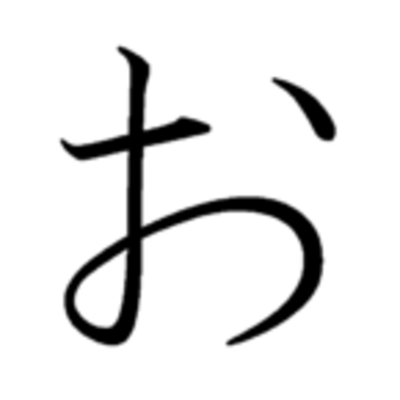
\includegraphics[scale=0.05]{KanaO}\ и 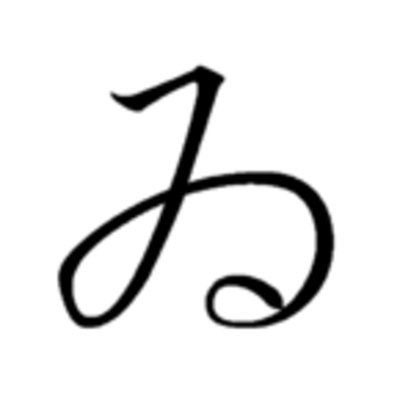
\includegraphics[scale=0.05]{KanaWi}}
    \end{figure}
    \item \emph{Цель работы: } построить и сравнить различные эвристики для исправления ошибок OCR, используя буквенную n-граммную модель японского языка.
\end{itemize}
\end{frame}

\begin{frame}
\frametitle{Текущие результаты}
\begin{itemize}
    \item Buckets
    \item NGram
    \item Backoff (+Katz)
    \item Zipf
\end{itemize}
\end{frame}

\begin{frame}
\frametitle{Список литературы}
\footnotesize{
\begin{itemize}
  \item Foundations of Statistical Natural Language Processing / \\C. D. Manning, H. Schutze.
  \item Efficient In-memory Data Structures for N-Grams Indexing / \\D. Robenek, J. Platos, V. Snasel
  \item Applying Conditional Random Fields to Japanese Morphological Analysis / T. Kudo, K. Yamamoto, Y. Matsumoto
\end{itemize}}
\end{frame}

\begin{frame}
\center{\huge
Спасибо
%\tiny\\
%\color{gray}
%Я пойду
}
\end{frame}

\end{document} 